\chapter{Datos y privacidad}\label{chap:datos}

En este capítulo se describen las fuentes de datos empleadas en el desarrollo del proyecto, así como sus principales características, alcance y utilidad dentro del proceso de análisis. La identificación y organización de estas fuentes resulta fundamental para comprender la base empírica sobre la cual se diseña, implementa y evalúa la solución propuesta. Asimismo, este inventario permite evidenciar la disponibilidad de información estructurada, documentos de soporte y metadatos de gestión necesarios para garantizar la trazabilidad del proceso y la validez de los resultados obtenidos.

\section{Análisis de datos}

El análisis de los datos es importante para fundamentar las decisiones de diseño e implementación de la solución propuesta. En esta sección se presentan las fuentes de información disponibles y cómo se organizan. En consecuencia, permite dimensionar el alcance del proyecto y las condiciones reales de operación. Posteriormente, se detalla la estructura del \textit{dataset} mediante un diccionario de datos y se examina la distribución de las variables más relevantes, con el objetivo de identificar patrones, limitaciones de calidad y oportunidades de mejora que orientan tanto la estrategia de extracción como la evaluación de resultados.

\subsection{Inventario de Fuentes de datos}

En este proyecto se emplean datos reales provenientes de la base operativa de una organización del sector \textit{fintech}, específicamente a partir de un respaldo de información almacenada en Airtable. El conjunto principal de datos comprende 316 registros de cuentas bancarias de instituciones educativas, recolectados entre septiembre de 2024 y abril de 2025. De estos registros, 308 cuentan con documentos de carátulas bancarias asociados, lo que representa una cobertura del 97.5\%. Esta alta proporción de registros con soporte de documentos resulta relevante, ya que permite desarrollar y evaluar la solución sobre información mayoritariamente completa, reduciendo la incertidumbre derivada de datos faltantes y fortaleciendo la validez del análisis. Adicionalmente, se dispone de otros tipos de documentos que podrían emplearse en futuras pruebas de generalización de la solución, entre ellos documentos de identidad mexicanos, facturas de ejemplo, comprobantes de domicilio y constancias de situación fiscal. En términos aproximados, se cuenta con alrededor de 50 documentos para cada una de las primeras tres categorías mencionadas, así como con más de 300 constancias de situación fiscal. Si bien estos documentos no fueron utilizados en la fase experimental del presente trabajo, su disponibilidad representa una base para evaluar en el futuro el comportamiento de la propuesta en escenarios de documentos distintos al caso inicial de validación bancaria.

Las fuentes de datos se organizan en tres categorías principales. En primer lugar, la base de datos en Airtable contiene 21 campos por registro con información estructurada de titulares, CLABEs, documentos de identificación (RFC/CURP), estados de validación y metadatos. Esta estructura proporciona una base sólida para contrastar la información extraída automáticamente con los datos operacionales ya existentes, lo que facilita la verificación de consistencia y calidad. En segundo lugar, los documentos de carátulas bancarias (308 archivos distribuidos en 220 PDFs, 35 JPGs, 34 PNGs y 19 en otros formatos) proporcionan la información visual necesaria para validar las cuentas. La diversidad de formatos resulta especialmente importante, ya que introduce condiciones heterogéneas de entrada similares a las que se presentan en un entorno real de operación, lo cual permite evaluar la robustez del sistema frente a distintos tipos de documentos. Finalmente, los metadatos de gestión incluyen fechas de creación, estados de procesamiento, identificadores de carpetas y \textit{logs} que permiten rastrear el flujo completo de cada registro. Esto aporta trazabilidad al proceso y posibilita no solo validar los resultados obtenidos, sino también identificar en qué etapa podrían producirse errores o inconsistencias dentro del flujo de procesamiento.

\subsection{Diccionario de datos y tamaños de bases de datos}

La Tabla~\ref{tab:diccionario_datos} presenta la estructura completa del \textit{dataset} con 21 campos de información bancaria, institucional y de gestión. En términos de volumen, el \textit{dataset} completo ocupa aproximadamente entre 150 y 200 MB, incluyendo tanto los datos estructurados como los documentos asociados. Esta dimensión resulta adecuada para el desarrollo del proyecto, ya que permite realizar procesos de exploración, validación y experimentación sin requerir una infraestructura computacional compleja, manteniendo al mismo tiempo un volumen suficientemente representativo de casos reales.

\begin{table}[htbp]
\centering
\begin{tabular}{p{3cm} p{2cm} p{5cm} p{4cm}}
\toprule
\textbf{Campo} & \textbf{Tipo} & \textbf{Descripción} & \textbf{Ejemplo} \\
\midrule
Nickname & String & Nombre descriptivo de la cuenta & CUENTA COLEGIATURAS \\
Owner & String & Titular de la cuenta bancaria & [NOMBRE\_TITULAR] \\
CLABE & String (18) & Clave Bancaria Estandarizada & [18 dígitos] \\
Currency & String & Moneda de la cuenta & MXN \\
document\_type & String & Tipo de documento de identificación & RFC, CURP \\
document\_number & String & Número del documento & [RFC/CURP] \\
banco & String & Nombre de la institución bancaria & BBVA MEXICO, BANORTE \\
school\_id & String & Identificador del colegio & SCH\#\#\# - [Nombre Colegio] \\
account\_type & String & Tipo de cuenta & CB (Cuenta Bancaria) \\
validation & String & Estado de validación & Completo, Incompleto \\
Colegio & String & Nombre completo del colegio & SCH\#\#\# - [Nombre Colegio] \\
school\_id (from Colegio) & UUID & Identificador único del colegio & [UUID] \\
Caratula & String & Nombre y URL del documento bancario & [archivo].pdf (https://...) \\
bank\_id & String & Identificador del banco (opcional) & (vacío) \\
drive\_folder\_id & String & ID de carpeta en Google Drive & [ID\_CARPETA] \\
created\_at & String & Fecha de creación & MM/DD/YYYY HH:MMam/pm \\
downloaded\_file & String & Nombre del archivo descargado localmente & row\#\#\#\_[nombre].ext \\
download\_status & String & Estado de descarga & success, no\_url \\
\bottomrule
\end{tabular}
\caption{Diccionario de datos del \textit{dataset} de cuentas bancarias}
\label{tab:diccionario_datos}
\end{table}


Un hallazgo relevante es la distribución de instituciones bancarias, ilustrada en la Figura~\ref{fig:distribucion_bancos}. De los 179 registros con banco identificado, BBVA concentra el 29\% de las cuentas, seguido por Banorte (16\%), Santander (15\%), Banamex (13\%), Scotiabank (9\%), Bajío (7\%), HSBC (3\%) y otros bancos (8\%). Esta distribución es importante porque permite identificar qué entidades financieras tienen mayor presencia en el conjunto analizado, lo que facilita priorizar pruebas y validaciones sobre los formatos bancarios más frecuentes y, en consecuencia, maximizar el impacto operativo de la solución propuesta.


Asimismo, se observa que el 56\% de los registros no tiene el campo de banco completado, lo que evidencia una limitación en la calidad del dataset. Este hallazgo no solo revela una oportunidad de mejora en los procesos de registro y validación de la información, sino que también justifica la utilidad de una solución automatizada capaz de extraer o inferir este dato a partir de los documentos asociados. En ese sentido, la distribución observada no solo refleja las preferencias del sector educativo mexicano al elegir instituciones financieras, sino que también pone de manifiesto brechas de calidad de datos que el proyecto puede contribuir a reducir.

\begin{figure}[htbp]
\centering
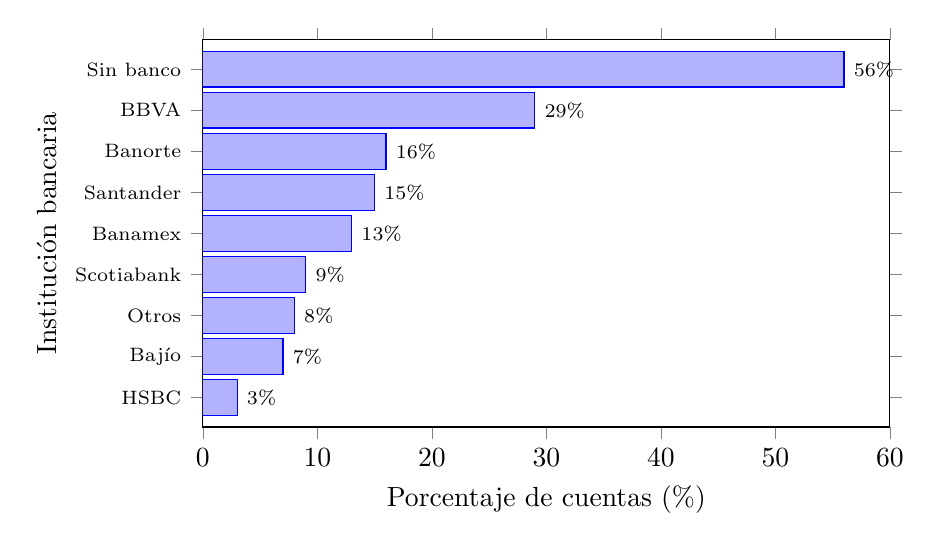
\begin{tikzpicture}
\begin{axis}[
    xbar,
    width=0.85\textwidth,
    height=6.5cm,
    bar width=0.45cm,
    xmin=0, xmax=60,
    xlabel={Porcentaje de cuentas (\%)},
    ylabel={Institución bancaria},
    symbolic y coords={HSBC,Bajío,Otros,Scotiabank,Banamex,Santander,Banorte,BBVA,Sin banco},
    ytick=data,
    yticklabel style={font=\scriptsize},
    nodes near coords,
    every node near coord/.append style={font=\scriptsize, color=black},
    nodes near coords align={horizontal},
    enlarge y limits=0.09,
    tick align=outside,
    axis line style={black},
    point meta=x,
    visualization depends on={x \as \rawx},
    nodes near coords={\pgfmathprintnumber{\rawx}\%},
]
\addplot coordinates {
    (3,HSBC)
    (7,Bajío)
    (8,Otros)
    (9,Scotiabank)
    (13,Banamex)
    (15,Santander)
    (16,Banorte)
    (29,BBVA)
    (56,Sin banco)
};
\end{axis}
\end{tikzpicture}
\caption{Distribución de registros por entidad bancaria dentro del \textit{dataset}}
\label{fig:distribucion_bancos}
\end{figure}

\subsection{Evaluación de Calidad}

El análisis de completitud del \textit{dataset} revela un panorama mixto. Mientras que el 97.5\% de los registros cuentan con carátula bancaria asociada, existen desafíos importantes en otros campos. El campo de banco presenta un 56\% de valores nulos, lo que dificulta el análisis por institución financiera y limita la posibilidad de segmentar los registros según la entidad bancaria correspondiente. Los campos de identificación del colegio (\texttt{school\_id}) muestran un 4.4\% de valores faltantes, mientras que las fechas de creación están ausentes en el 18.4\% de los registros, afectando la trazabilidad temporal del \textit{dataset} y el seguimiento del flujo de procesamiento. En conjunto, estos resultados evidencian que, aunque la disponibilidad de documentos es alta, la calidad de ciertos atributos estructurados aún presenta debilidades que pueden impactar el análisis y la validación de resultados. Por ello, la identificación de valores faltantes no solo permite diagnosticar el estado actual del dataset, sino también justificar la necesidad de incorporar estrategias de limpieza, enriquecimiento y validación de datos dentro del proyecto. La Figura~\ref{fig:porcentaje_nulos} detalla el porcentaje de valores faltantes para los campos más relevantes del dataset.


\begin{figure}[htbp]
\centering
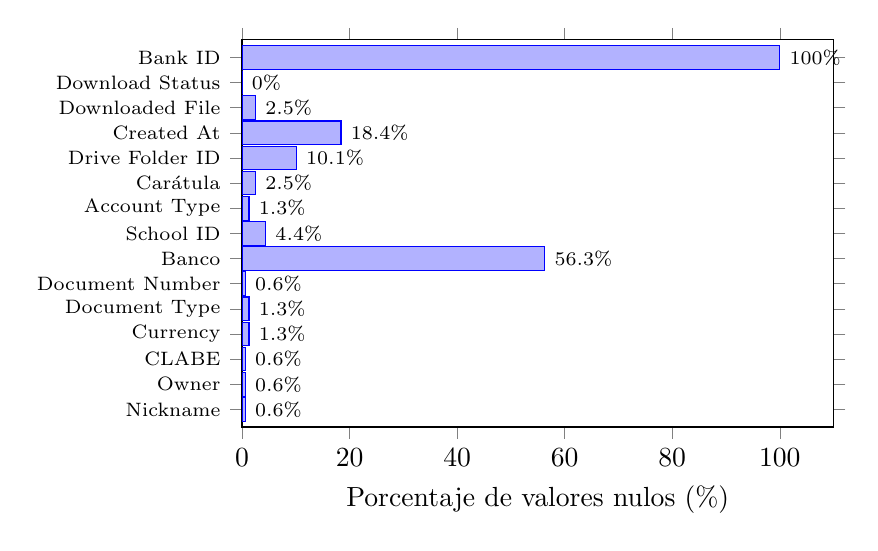
\begin{tikzpicture}
\begin{axis}[
    xbar,
    width=0.75\textwidth,
    height=6.5cm,
    bar width=0.3cm,
    xmin=0, xmax=110,
    xlabel={Porcentaje de valores nulos (\%)},
    symbolic y coords={
        Nickname,
        Owner,
        CLABE,
        Currency,
        Document Type,
        Document Number,
        Banco,
        School ID,
        Account Type,
        Carátula,
        Drive Folder ID,
        Created At,
        Downloaded File,
        Download Status,
        Bank ID
    },
    ytick=data,
    yticklabel style={font=\scriptsize},
    point meta=x,
    visualization depends on={x \as \rawx},
    nodes near coords={\pgfmathprintnumber{\rawx}\%},
    nodes near coords align={horizontal},
    every node near coord/.append style={font=\scriptsize, color=black},
    enlarge y limits=0.05,
    tick align=outside,
    axis line style={black},
]
\addplot coordinates {
    (0.6,Nickname)
    (0.6,Owner)
    (0.6,CLABE)
    (1.3,Currency)
    (1.3,Document Type)
    (0.6,Document Number)
    (56.3,Banco)
    (4.4,School ID)
    (1.3,Account Type)
    (2.5,Carátula)
    (10.1,Drive Folder ID)
    (18.4,Created At)
    (2.5,Downloaded File)
    (0.0,Download Status)
    (100.0,Bank ID)
};
\end{axis}
\end{tikzpicture}
\caption{Porcentaje de valores nulos por campo en el \textit{dataset}.}
\label{fig:porcentaje_nulos}
\end{figure}

En cuanto a los duplicados (Figuras~\ref{fig:titulares_duplicados} y~\ref{fig:clabe_duplicadas}), se identificaron 29 CLABEs repetidas que involucran a 66 registros (20.9\% del total), así como titulares duplicados en aproximadamente el 36\% de los casos (114 registros). No obstante, estos valores no deben interpretarse necesariamente como errores de calidad de datos. En muchos casos, corresponden a instituciones educativas que mantienen múltiples cuentas bancarias o registran una misma cuenta para distintos conceptos, como colegiaturas, inscripciones o facturación. Este patrón resulta consistente con la lógica operativa del sector educativo, donde una misma institución puede requerir diversas configuraciones administrativas y financieras. Por ello, la presencia de duplicados en estos campos no solo debe analizarse desde una perspectiva técnica, sino también considerando el contexto funcional en el que los registros son utilizados.


\begin{figure}[H]
    \centering
    \begin{minipage}{0.42\textwidth}
        \centering
        {\footnotesize Duplicados en titulares}
        
        \begin{tikzpicture}
            \pie[
                radius=1.5,
                text=inside,
                after number=\%,
                color={blue!20, blue!40},
                sum=100
            ]{64.0/, 36.0/}
        \end{tikzpicture}

        {\scriptsize
        \textcolor{blue!20}{\rule{0.3cm}{0.3cm}} Titulares únicos \quad
        \textcolor{blue!40}{\rule{0.3cm}{0.3cm}} Titulares duplicados
        }
        
        \caption{Distribución de titulares únicos y duplicados en el \textit{dataset} analizado.}
        \label{fig:titulares_duplicados}
    \end{minipage}
    \hfill
    \begin{minipage}{0.42\textwidth}
        \centering
        {\footnotesize Duplicados en CLABE}
        
        \begin{tikzpicture}
            \pie[
                radius=1.5,
                text=inside,
                after number=\%,
                color={blue!20, blue!40},
                sum=100
            ]{79.1/, 20.9/}
        \end{tikzpicture}

        {\scriptsize
        \textcolor{blue!20}{\rule{0.3cm}{0.3cm}} Únicas \quad
        \textcolor{blue!40}{\rule{0.3cm}{0.3cm}} CLABEs duplicadas
        }
        
        \caption{Distribución de CLABEs únicas y duplicadas en el \textit{dataset} analizado.}
        \label{fig:clabe_duplicadas}
    \end{minipage}
\end{figure}

El análisis también reveló algunas anomalías que requieren atención antes de utilizar los datos para la evaluación de modelos de lenguaje. Se encontró un registro con CLABE en formato incorrecto (marcado como ``CLABE incorrecta'' en el campo de validación), varios números de cuenta con caracteres especiales (apóstrofes, comillas y espacios embebidos), 8 documentos que no pudieron descargarse (2.5\% del total, marcados como ``no\_url''), formatos de fecha inconsistentes que necesitan normalización y un alto porcentaje de registros con el campo de banco sin completar (56.3\%). Estas incidencias evidencian la necesidad de incorporar una etapa de limpieza, normalización y validación previa al entrenamiento, ya que la calidad de los datos de entrada influye directamente en el desempeño y la confiabilidad de los resultados.


A pesar de ello, el análisis también muestra que el \textit{dataset}presenta características favorables para el proyecto. Se observa una cobertura geográfica nacional que abarca múltiples estados de México, una alta disponibilidad de documentos con 97.5\% de carátulas descargadas exitosamente y un 43.4\% de cuentas marcadas como ``Completo'' en su validación. Aunque el 56.3\% de los registros aparecen como ``Incompleto'', esta condición se explica principalmente por la ausencia del campo de banco y no por la falta de documentación asociada. Esto resulta especialmente relevante, ya que los documentos de carátulas bancarias constituyen la fuente principal para la evaluación de los modelos de extracción automática. En consecuencia, las anomalías identificadas no invalidan el uso del dataset, sino que delimitan con mayor claridad las tareas de preprocesamiento necesarias y confirman que se dispone de una base robusta y suficientemente representativa para desarrollar la solución propuesta.


\section{Cumplimiento de Privacidad de Datos}

El proyecto trabaja con datos personales y financieros, lo que exige un tratamiento responsable desde el diseño del sistema. En esta sección se presenta el marco legal que aplica al proyecto y se identifica qué información es sensible. Se describen también los flujos de datos, los riesgos de privacidad detectados y las acciones tomadas para cumplir con la normativa vigente.

\subsection{Marco legal aplicable}

Dado que el proyecto maneja información financiera y personal sensible, debe cumplir con un marco regulatorio estricto. En primer lugar, la Ley Federal de Protección de Datos Personales en Posesión de los Particulares (LFPDPPP) establece los principios fundamentales para el tratamiento de datos personales en México, incluyendo los derechos ARCO (Acceso, Rectificación, Cancelación y Oposición) que deben garantizarse a los titulares. Adicionalmente, los Lineamientos del Aviso de Privacidad publicados por el INAI (Instituto Nacional de Transparencia, Acceso a la Información y Protección de Datos Personales) especifican cómo debe informarse a los usuarios sobre el uso de sus datos. Finalmente, al tratarse de información bancaria, también aplican los Estándares de seguridad establecidos por la CNBV (Comisión Nacional Bancaria y de Valores), que regulan el manejo de información financiera sensible en el sector.

\subsection{Identificación de Información Personal Identificable (PII)}

El \textit{dataset} contiene múltiples categorías de información personal identificable (PII) \cite{nist_pii} que requieren protección especial. Los campos más sensibles, por un lado, incluyen las CLABEs (números de cuenta bancaria de 18 dígitos), los números de documento (RFC/CURP) y los nombres de los titulares de las cuentas. Estos datos críticos requieren medidas de seguridad robustas como tokenización y encriptación. Por otro lado, campos de sensibilidad media como los identificadores de colegios y nombres de instituciones requieren pseudonimización para proteger la privacidad sin perder la utilidad de los datos. La Tabla~\ref{tab:clasificacion_pii} presenta la clasificación completa de PII por nivel de sensibilidad y las medidas de protección requeridas para cada categoría.

\begin{table}[H]
\centering
\begin{tabular}{l l l p{4.5cm}}
\toprule
\textbf{Campo} & \textbf{Categoría} & \textbf{Riesgo} & \textbf{Medidas requeridas} \\
\midrule
\multicolumn{4}{c}{\textbf{PII Directa (Alta sensibilidad)}} \\
\midrule
Owner & Nombre completo & Alto & Anonimización, encriptación \\
CLABE & Datos financieros & Crítico & Tokenización, encriptación en reposo \\
document\_number & Identificador fiscal/personal & Crítico & Enmascaramiento, acceso restringido \\
Caratula (URL) & Documento bancario & Crítico & Control de acceso, encriptación \\
\midrule
\multicolumn{4}{c}{\textbf{PII Indirecta (Sensibilidad media)}} \\
\midrule
Nickname & Identificador descriptivo & Medio & Revisar caso por caso \\
school\_id & Afiliación institucional & Medio & Pseudonimización \\
Colegio & Nombre de institución & Medio & Puede revelar ubicación \\
banco & Institución financiera & Bajo & Dato semi-público \\
\midrule
\multicolumn{4}{c}{\textbf{Metadatos sensibles}} \\
\midrule
drive\_folder\_id & Ubicación de documentos & Medio & Control de acceso, auditoría \\
downloaded\_file & Ruta de archivo local & Bajo & Protección del sistema de archivos \\
created\_at & Timestamp de actividad & Bajo & Análisis de patrones \\
\bottomrule
\end{tabular}
\caption{Clasificación de PII por nivel de sensibilidad}
\label{tab:clasificacion_pii}
\end{table}

\subsection{Mapa de flujo de datos (Data Flow Map)}

Para garantizar la privacidad desde el diseño, resulta fundamental mapear el flujo completo de los datos a través del sistema. La figura~\ref{fig:data_flow} ilustra este recorrido en cinco etapas principales. En primer lugar, los datos se originan en Airtable y Google Drive, donde la organización analizada almacena información operacional y de documentos. En segundo lugar, pasan por una etapa de procesamiento que incluye descarga, \textit{parsing} y anonimización propuesta. Posteriormente, en tercer lugar, se almacenan en reposo tanto los datos estructurados como los documentos originales. En la cuarta etapa, los datos se emplean para la evaluación y validación de los modelos de \textit{machine learning}. Finalmente, se aplica una política de retención de cinco años, asociada a requerimientos de cumplimiento fiscal, seguida de procesos de eliminación segura. Cada una de estas etapas incorpora puntos de control específicos orientados a la protección de la privacidad.

\begin{figure}[H]
\centering
\small
\begin{tikzpicture}[
    box/.style={
        draw=gray!60,
        fill=gray!3,
        rounded corners=4pt,
        text width=10.3cm,
        inner sep=7pt,
        font=\small,
        align=left
    },
    arrow/.style={
        ->,
        thick,
        gray!55
    },
    node distance=0.55cm
]

\node[box] (n1) {
    \textbf{1. Fuentes de datos}\\
    • Airtable: registros con datos bancarios y metadatos\\
    • Google Drive: documentos en PDF e imagen\\
    {\scriptsize \textit{Control: acceso restringido al equipo autorizado}}
};

\node[box, below=of n1] (n2) {
    \textbf{2. Procesamiento y protección}\\
    • Descarga y consolidación de documentos\\
    • Extracción de campos relevantes\\
    • Tokenización, enmascaramiento y pseudonimización\\
    {\scriptsize \textit{Control: tratamiento de datos antes de evaluación de modelos}}
};

\node[box, below=of n2] (n3) {
    \textbf{3. Almacenamiento}\\
    • Datos estructurados y documentos originales\\
    • Resultados, métricas y trazabilidad del flujo\\
    {\scriptsize \textit{Control: cifrado y resguardo conforme a normativa aplicable}}
};

\node[box, below=of n3] (n4) {
    \textbf{4. Evaluación y validación}\\
    • Evaluación de modelos de extracción sobre documentos\\
    • Métricas de precisión y análisis de errores\\
    {\scriptsize \textit{Control: módulo de anonimización para tokenización, enmascaramiento y pseudonimización}}
};

\node[box, below=of n4] (n5) {
    \textbf{5. Retención y eliminación}\\
    • Política de retención de 5 años (cumplimiento fiscal)\\
    • Eliminación segura al cumplir el propósito del tratamiento\\
    {\scriptsize \textit{Control: endpoint de eliminación + purga automática conforme a LFPDPPP}}
};

\draw[arrow] (n1) -- (n2);
\draw[arrow] (n2) -- (n3);
\draw[arrow] (n3) -- (n4);
\draw[arrow] (n4) -- (n5);

\end{tikzpicture}
\caption{Flujo general de datos y controles de privacidad.}
\label{fig:data_flow}
\end{figure}
\subsection{Privacidad desde el diseño}

El tratamiento de la información sensible se plantea bajo principios de seguridad, confidencialidad y uso responsable de los datos personales. Este enfoque busca garantizar que la información sea procesada de manera controlada y permanezca protegida durante todo su ciclo de vida. En ese marco, se aplica el principio de minimización de datos, de modo que solo se recopilan los campos estrictamente necesarios para la validación bancaria, sin almacenar información adicional más allá de la requerida por el proceso operativo, en concordancia con las prácticas de tratamiento de información personal descritas por el NIST para PII \cite{nist_pii}. Del mismo modo, se cumple con la limitación de propósito, garantizando que los datos recopilados se utilicen exclusivamente para la validación de cuentas bancarias y no sean compartidos con terceros sin el consentimiento explícito del titular, tal como lo establece el artículo 12 de la LFPDPPP \cite{lfpdppp}.

Asimismo, se implementan técnicas de anonimización orientadas a reducir el riesgo de exposición de datos personales. Entre ellas se incluyen la tokenización de CLABEs, mediante la sustitución de los números de cuenta por identificadores numéricos no reversibles generados con SHA-256; el enmascaramiento de RFC y CURP, a través de la ocultación parcial de caracteres conservando únicamente los extremos del identificador; y la pseudonimización de nombres, reemplazándolos por identificadores determinísticos genéricos. A ello se suman medidas de seguridad que garantizan la encriptación tanto en tránsito como en reposo: durante la transmisión de datos se emplea el protocolo HTTPS/TLS reforzado con cabeceras de seguridad (HSTS, X-Content-Type-Options, X-Frame-Options, CSP), mientras que para el almacenamiento en reposo se utiliza cifrado a nivel de campo mediante el esquema Fernet (AES en modo CBC con HMAC-SHA256) para los campos sensibles de los registros de extracción. Finalmente, se aplican mecanismos de control de acceso basados en el modelo RBAC (\textit{Role-Based Access Control}) con tres roles diferenciados, junto con un módulo de auditoría que registra los accesos a \textit{endpoints} sensibles (incluyendo el identificador del usuario, la acción realizada, la dirección IP y la marca temporal) y autenticación multifactor heredada de las configuraciones de cada usuario en GitHub OAuth \cite{nist_pii}.\vspace{-1.8em}

\subsubsection{Anonimización para el procesamiento con modelos de \textit{Document Understanding}}

Dado que la solución emplea modelos de lenguaje a través de una API externa (Claude) y no realiza un entrenamiento de modelos propio, los documentos son enviados al servicio para su procesamiento en tiempo real. En este contexto, el sistema incorpora un módulo de anonimización estructurada \cite{google_docunderstanding} que permite eliminar o transformar la información personal identificable antes de su uso en tareas de evaluación, análisis o mejora del sistema.

El procedimiento sigue la siguiente secuencia:
\begin{tcolorbox}[
    colback=gray!5,
    colframe=gray!50,
    title={Proceso de anonimización implementado},
    fonttitle=\bfseries,
    sharp corners,
    boxrule=0.5pt
]
\small

\textbf{Flujo de anonimización:}

\begin{center}
\fbox{\parbox{3cm}{\centering Documento\\original}}
$\rightarrow$
\fbox{\parbox{3cm}{\centering Extracción\\de texto}}
$\rightarrow$
\fbox{\parbox{3cm}{\centering Identificación\\de PII}}
$\rightarrow$
\fbox{\parbox{3cm}{\centering Reemplazo\\por tokens}}
\end{center}

\vspace{6pt}

\begin{tabular}{ll}
\textbf{Texto original} & \textbf{Texto anonimizado} \\[6pt]

\texttt{Titular: [NOMBRE COMPLETO]} &
\texttt{Titular: [NOMBRE\_PERSONA]} \\

\texttt{RFC: [13 CARACTERES ALFANUMÉRICOS]} &
\texttt{RFC: [RFC\_ID]} \\

\texttt{CLABE: [18 DÍGITOS NUMÉRICOS]} &
\texttt{CLABE: [CLABE\_18\_DIGITOS]} \\
\end{tabular}

\vspace{4pt}



\end{tcolorbox}

\noindent Este proceso preserva la estructura y el formato del documento, manteniendo patrones propios de los campos bancarios y fiscales, como la longitud esperada de la CLABE y del RFC, así como la posición espacial y los elementos visuales presentes, entre ellos tablas y logotipos. Adicionalmente, las funciones de anonimización permiten generar versiones anonimizadas de los resultados de extracción, donde los nombres se reemplazan por pseudónimos determinísticos, las CLABEs se sustituyen por tokens numéricos no reversibles y los RFC y CURP se enmascaran parcialmente. Ello permite evaluar los modelos sobre datos representativos, reduciendo al mismo tiempo el riesgo asociado al uso directo de información sensible.

La implementación de este proceso se respalda con medidas de seguridad estructuradas en tres niveles complementarios: aplicación, infraestructura y organización. En el nivel de aplicación, se implementan validaciones de entrada mediante Pydantic, cifrado de campos sensibles mediante Fernet, y registros de auditoría sobre las operaciones que involucran información personal identificable. En el nivel de infraestructura, se contempla el almacenamiento de datos en servidores con cifrado en tránsito (HTTPS/TLS) y cabeceras de seguridad, junto con controles de acceso basados en URLs prefirmadas. Por último, en el nivel organizacional, se consideran la capacitación continua del personal, la firma de acuerdos de confidencialidad y la implementación de procedimientos de respuesta ante incidentes.

\subsubsection{Requerimientos relacionados con la privacidad de datos}

Las medidas descritas en esta sección constituyen la base operativa del enfoque de privacidad desde el diseño aplicado en el proyecto. Cada acción implementada corresponde a un requerimiento técnico que orienta el manejo de la información sensible dentro del sistema. La Tabla~\ref{tab:requerimientos_privacidad} presenta la formalización de estos requerimientos de privacidad, los cuales aseguran que las medidas adoptadas puedan verificarse y mantenerse.

\begin{table}[H]
    \centering
    \resizebox{0.9\textwidth}{!}{%
    \begin{tabular}{p{1.2cm} p{10cm} p{3cm}}
    \toprule
    \textbf{Código} & \textbf{Descripción} & \textbf{Tipo} \\
    \midrule
    R-01 & Cifrado de CLABE, RFC y CURP en tránsito (HTTPS/TLS) y en reposo (Fernet AES-CBC con HMAC-SHA256) mediante estándares de seguridad avanzados. & No funcional \\
    R-02 & Implementación de control de acceso basado en roles (RBAC) y auditoría de accesos a datos sensibles para limitar y rastrear el acceso a información crítica. & Funcional \\
    R-03 & Gestión del consentimiento informado de los titulares de los datos, permitiendo su revocación en cualquier momento mediante \textit{endpoints} dedicados. & Funcional \\
    R-04 & Aplicación de anonimización y seudonimización automática mediante tokenización, enmascaramiento y pseudonimización antes del uso de datos en evaluación. & No funcional \\
    R-05 & Eliminación segura de los datos personales una vez cumplido el propósito del tratamiento, con política de retención de cinco años y mecanismo de purga. & No funcional \\
    \bottomrule
    \end{tabular}
    }
    \caption{Requerimientos relacionados con la privacidad de datos}
    \label{tab:requerimientos_privacidad}
\end{table}

\subsubsection{Historias de usuarios relacionadas con la privacidad de datos}

La siguiente sección presenta historias de usuario que reflejan cómo los diferentes actores del sistema interactúan con los mecanismos de protección de datos personales, en cumplimiento con los principios de confidencialidad, minimización y control de acceso establecidos en el diseño del sistema.  
Estas historias permiten traducir los requerimientos legales y técnicos de privacidad en funcionalidades específicas dentro de la arquitectura del proyecto.

\begin{itemize}
    \item \textbf{HU-01: Control de acceso y confidencialidad.}  
    Como administrador del sistema, quiero que los usuarios solo puedan acceder a la información necesaria según su rol, para garantizar la protección de datos sensibles presentes en documentos financieros y administrativos, mediante mecanismos de control de acceso basado en roles y el cumplimiento del principio de mínimo privilegio.

    \item \textbf{HU-02: Tratamiento seguro de datos sensibles.}  
    Como miembro del equipo de datos, quiero que el sistema aplique mecanismos de anonimización u ofuscación sobre la información contenida en los documentos cuando estos sean utilizados para procesos de evaluación, análisis o mejora del sistema, con el fin de evitar la exposición de información personal identificable (PII).

    \item \textbf{HU-03: Consentimiento y trazabilidad del uso de datos.}  
    Como titular de los datos, quiero poder otorgar y revocar mi consentimiento para el uso de mi información en procesos de validación o análisis, así como contar con mecanismos de trazabilidad que permitan auditar su uso, a fin de asegurar que el tratamiento se realice conforme a la normativa vigente en materia de protección de datos.
\end{itemize}
\subsection{Evaluación de riesgos de privacidad}

La evaluación de riesgos de privacidad tiene como propósito identificar los posibles eventos que podrían afectar la confidencialidad, integridad o disponibilidad de los datos personales tratados por el sistema. Este análisis permite estimar la probabilidad de ocurrencia y el impacto de cada riesgo, con el fin de priorizar las medidas de mitigación más adecuadas. La Tabla~\ref{tab:riesgos_privacidad} resume los principales riesgos identificados durante el diseño y desarrollo del sistema, junto con el nivel de probabilidad, el impacto potencial y las medidas de mitigación implementadas.

El análisis evidencia que los riesgos de mayor criticidad se relacionan con la posible exposición de CLABEs en los datos de evaluación y con la reidentificación de datos anonimizados. El MVP mitiga estos riesgos mediante la tokenización de campos numéricos sensibles, el cifrado a nivel de campo en la base de datos, el control de acceso basado en roles, la auditoría de accesos y las utilidades de pseudonimización. En consecuencia, el conjunto de medidas implementadas refuerza la protección de los datos personales y contribuye a mantener un equilibrio adecuado entre seguridad, eficiencia y cumplimiento normativo.

\begin{table}[H]
\centering
\begin{tabular}{p{3.5cm} l l p{7cm}}
\toprule
\textbf{Riesgo} & \textbf{Probabilidad} & \textbf{Impacto} & \textbf{Mitigación implementada} \\
\midrule
Fuga de CLABEs en datos de evaluación & Media & Crítico & Tokenización de CLABEs mediante módulo de anonimización; cifrado de campos en reposo \\
Acceso no autorizado a documentos bancarios & Baja & Alto & RBAC + cifrado a nivel de campo + URLs prefirmadas con expiración \\
Re-identificación a partir de datos anonimizados & Baja & Alto & Pseudonimización determinística + enmascaramiento parcial de RFC/CURP \\
Pérdida de datos por fallo de hardware & Media & Medio & Respaldos gestionados por el proveedor de infraestructura (Railway/PostgreSQL) \\
Uso indebido por personal interno & Baja & Alto & RBAC + auditoría de accesos a datos sensibles + principio de mínimo privilegio \\
\bottomrule
\end{tabular}
\caption{Evaluación de riesgos de privacidad}
\label{tab:riesgos_privacidad}
\end{table}


\subsection{Cumplimiento y auditoría}

El aviso de privacidad informa a los colegios y a los titulares sobre los datos recopilados, su finalidad, el uso de inteligencia artificial para el procesamiento automatizado, los derechos ARCO (Acceso, Rectificación, Cancelación y Oposición) y el periodo de retención correspondiente. Asimismo, se requiere el consentimiento informado y explícito para el procesamiento automatizado de documentos bancarios, el almacenamiento temporal de carátulas y el uso de datos para la evaluación de modelos. Para ello, el sistema implementa un mecanismo de gestión del consentimiento que permite registrar, consultar y revocar el consentimiento de cada usuario mediante \textit{endpoints} dedicados. Por su parte, las auditorías periódicas comprenden el registro automático de accesos a datos sensibles en una tabla de auditoría, la revisión trimestral de dichos registros, la evaluación anual de las medidas de seguridad y la ejecución de pruebas de penetración semestrales. En complemento, el derecho al olvido se implementa mediante un \textit{endpoint} que permite al usuario solicitar la eliminación de todos sus datos de extracción, conforme a la LFPDPPP, e incluye la eliminación de la información en todos los sistemas involucrados. Adicionalmente, se implementa una política de retención de datos con un periodo de cinco años asociado a requerimientos de cumplimiento fiscal, con un mecanismo administrativo para la purga de registros expirados. Estas medidas resultan fundamentales porque no solo permiten cumplir con las obligaciones legales aplicables, sino que también refuerzan la confianza de los titulares y reducen los riesgos asociados al tratamiento automatizado de información sensible.


